\chapter{Analysis}\label{ch:analysis}

\section{Results}
This section makes an assessment of the final product and its results by pointing out what went well and what could be improved.  


\subsection{Evaluation}
%\begin{itemize}
%\item \colorbox{pink}{do we think we are successful?}
%\item \colorbox{pink}{did we manage to do what we wanted?}
%\item \colorbox{pink}{did we prove what we wanted to prove?}
%\item \colorbox{pink}{is it really a useful tool?}
%\item \colorbox{pink}{who is it targeting as a user?}
%\end{itemize} 

Overall, the work of this thesis proved successful. Procedural audio is used to replace prerecorded sound effects in a virtual environment. The sounds are generated using modal synthesis and based on physical models which are excited by different interactions driven by physics events in the game engine. The tool implemented enables the sound designer to control the synthesizer by choosing different materials for every object, the roughness of its surface and size.

\paragraph{Sounding objects\\}
The tool provides ready-made Unity\textsuperscript{\textregistered} prefabs and their corresponding audio components attached. The sounds produced by the proposed prefabs are object-specific, meaning that the modal data they have assigned matches their physical properties. The effect of this is a sound which is tightly coupled with its corresponding audio source. However, one can use the modal data of a certain object for a different shaped object, if it fits their needs. 

A drawback that entails from the aforementioned is that incorporating new objects in the game scene that can benefit from the tool is not a straightforward task. To ease the process a detailed guide that walks through the steps to add new objects and obtain their modal parameters is available in the appendix \ref{ap:guide}. 

\paragraph{Sound variation\\}
Since objects were separated into different sounding areas, it was easier to assume that all materials are homogeneous and isotropic. This assumption decreases the realistic aspect of sound variation along an object's surface which would ideally produce a different sound in every location. The higher resolution of the object's surface the more accurate will the sound on its surface be. This however results in higher calculations and higher amount of necessary recordings for every one of the areas. Therefore, a compromise is needed between the amount of ``sound areas'' and the realism of the varying sound. Section \ref{sec:discretization} explained how the objects were divided into areas with a heuristic approach. The sounds generated by the objects within a virtual scene are compelling from the point of view of the authors and thus validated this approach.



\paragraph{Synthetic sounds versus recordings\\}

Regarding the quality of the synthesized sounds it can be said that in general, sounds that present high damping are less suitable for modal synthesis than sounds with low damping. 

Sounds produced by highly damped materials such as plastic or wood present spectrograms where information is spread in a wide frequency range. In this thesis the ten most prominent modes were chosen which leads to loss of information and thus a decrease in the richness of the sound. Nevertheless, it was possible to synthesize sounds coming from these types of objects. For example, the wooden cutting board, used in this study, is broad in frequency domain as seen in the first row of figure \ref{fig:specs_cb}. However, the synthesized sounds' spectrograms show that our method is able to keep the most important information despite some frequency components loss. 

On the other hand, sounds coming from low damped materials such as glass or metal present very clear frequency peaks. As seen in the spectrograms of the wine glass recordings in the appendix \ref{ap:spectrograms}, few peaks stand out among the rest. For this reason most of the information can be synthesized within ten modes. It can be seen on the spectrograms corresponding to the synthetic sounds of the wine glass that the prominent peaks are present. This is also validated also through unofficial auditory perception tests. 


\begin{figure}[H]
  \centering
    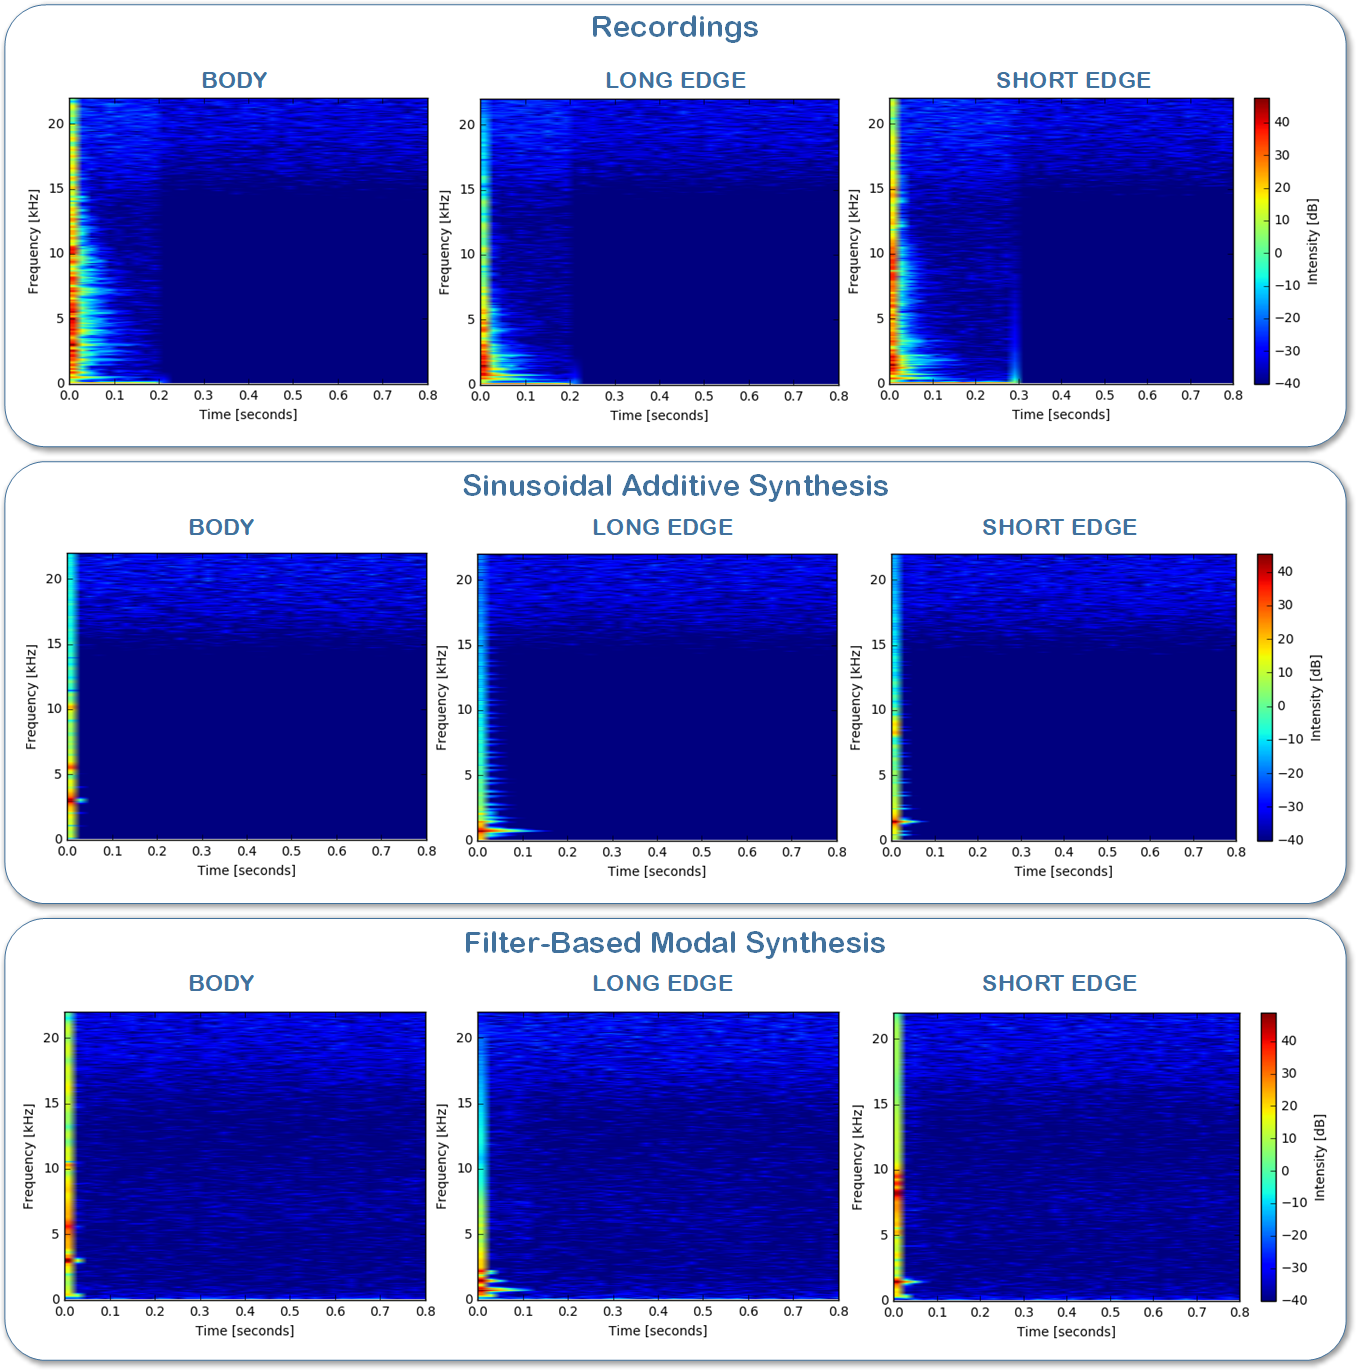
\includegraphics[width=\textwidth]{specs/cb_rec_sin.png}
      \caption{Spectrograms of a cutting board object's real-wolrd recordings and synthesized impacts, using sinusoidal additive synthesis.}
      \label{fig:specs_cb}
\end{figure}

Without leaving the realm of low damped materials, it is worth mentioning that in some cases metallic sounds cause undesired distortions. More specifically, for Q-factor values over $3100$, a distorted sound can be heard when the object is hit in different areas  in a short time-lapse. The origin of this problem seems to be the change of the modal frequencies (as certain areas have different modes than others) that are fed into the filters while the previous sound is still ``ringing''. 


Other inaccuracies in the synthetic sounds may derive from both the recording and parameters extraction phase. This thesis does not calculate the residual sound, namely the differentiation between the real-world sound and the synthesized sound \cite{ren2013example}. Therefore, information that concerns mostly the beginning of the sound (when the collision happens) is not calculated and is said to be perceptually relevant to identify the sounding object \cite{freed1990auditory}. However, the reason it was not included was precisely because we did not want the noise produced by the striker (a drumstick in this case) to be present in the synthesized sound. This is because in the game scene the characteristics of the striking object are unknown. Another aspect that could have affected the synthetic sounds is again the sound of the drumstick that may have interfered in the data extraction phase.

Using procedural audio in games is much more convenient and less expensive as far as storage space is concerned compared to the use of audio files. In this paper the plugins corresponding to the filter-based synthesis method occupy 523 kB while the ones for the sinusoidal method are 772 kB. The total memory needed to store the recordings of the struck objects is 5.74 MB. The space saved with the synthesis techniques is indisputable. Moreover, procedural audio is adaptive to several different scenarios without further change or additional memory needs, as it is flexible and dynamic. For example, with just a slider, size adjustment is achieved.  Adding new sounds is less time consuming and it is better for mobile platforms that are limited in both storage space and computational power.

\paragraph{Controlling parameters\\}

The tool itself is easy-to-use with the already existing objects as one can control sound properties through high level parameters that are intuitive for the user. Those controllers which are explained in section \ref{sec:UI} are neither \textit{weak} nor too \textit{strong}. As stated in \cite{jaffe1995ten}, weak parameters affect the result so little, that there is a possibility the designer will adjust them to arbitrary values as he is ``wandering in the dark''. On the other hand, when even a minuscule tweaking of a very strong parameter induces a big change, the designer will probably find it difficult to choose the value he wants. In this thesis certain functions were used to offer coherent sliders that allow an efficient control.

Using the provided Unity\textsuperscript{\textregistered} prefabs as reference, the same modal data can be transferred automatically to reflect variations in object scaling or surface roughness and between different materials assigned to the same object. Spectrograms of the synthesized sound produced by a struck cup with different sizes (from smaller to bigger) can be seen in figure \ref{fig:cup_sizes}. Resonant frequencies are inversely proportional to the size, thus the pitch goes down when the object gets bigger.

Figure \ref{fig:bottle_rough} displays waveforms of a rolling bottle with different surface roughness values. As the roughness parameter is increased, the sound generated by the bumps along the surface becomes more audible. It is noticeable by looking at the waveforms that the rougher the surface the louder the synthetic sounds derived from the micro-collisions are. This evidence matches with the graph \ref{fig:roughnessgraph} from section \ref{sec:rolling_synth} that shows how the amplitude of the impulses corresponding to the bumps increases with the roughness of the object. An improvement to customize the surface irregularity of the object would be to implement a two dimensional graph that maps the object's contour profile with a curve (similarly to the curves in \ref{fig:roughnessgraph}). This way the user could fine-tune the roughness of the object with a more visual controller.

Figure \ref{fig:bottle_materials} shows spectrograms of a bottle falling over several platforms with different materials assigned to it, starting from plastic on the left and ending with metal on the right. Although the impact sounds are produced at the same moment of time, it can be seen that the ``tails'' of the individual impacts last longer towards the rightmost spectrogram which corresponds to metal. This proves the fact that the lower the damping (as for metallic sounds) the longer the sound lasts.

All controllers offer the possibility to be modified at run-time which is an advantage as changes in sound can be experimented on the go. Despite this, some small disturbances can be heard when controlling the \textit{Size} slider as it modifies the central frequencies of the filters or the oscillators as a sound is already ``ringing''.

\begin{figure}[H]
  \centering
    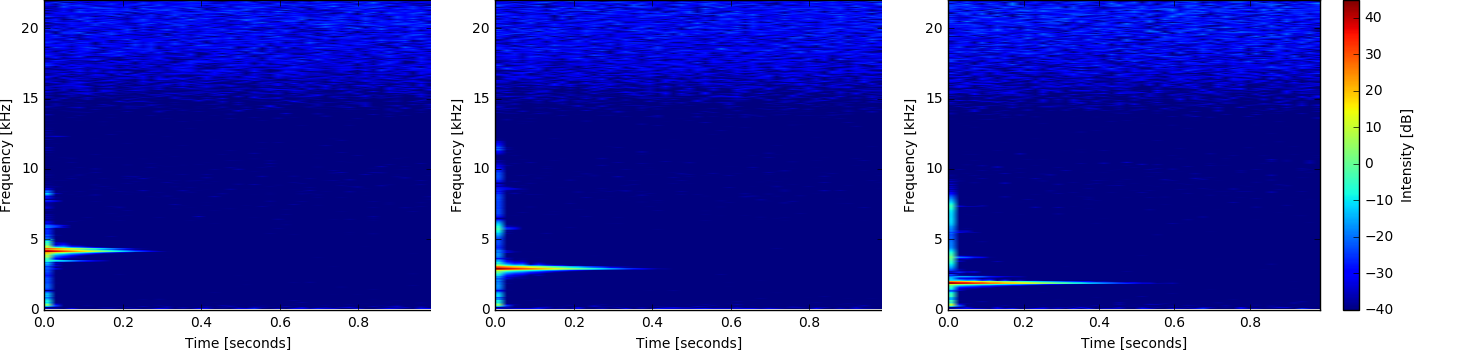
\includegraphics[width=\textwidth]{specs/cup_sizes.png}
      \caption{Spectrograms of a cup object with size variation (smaller, reference size and bigger respectively).}
      \label{fig:cup_sizes}
\end{figure}

\begin{figure}[H]
  \centering
    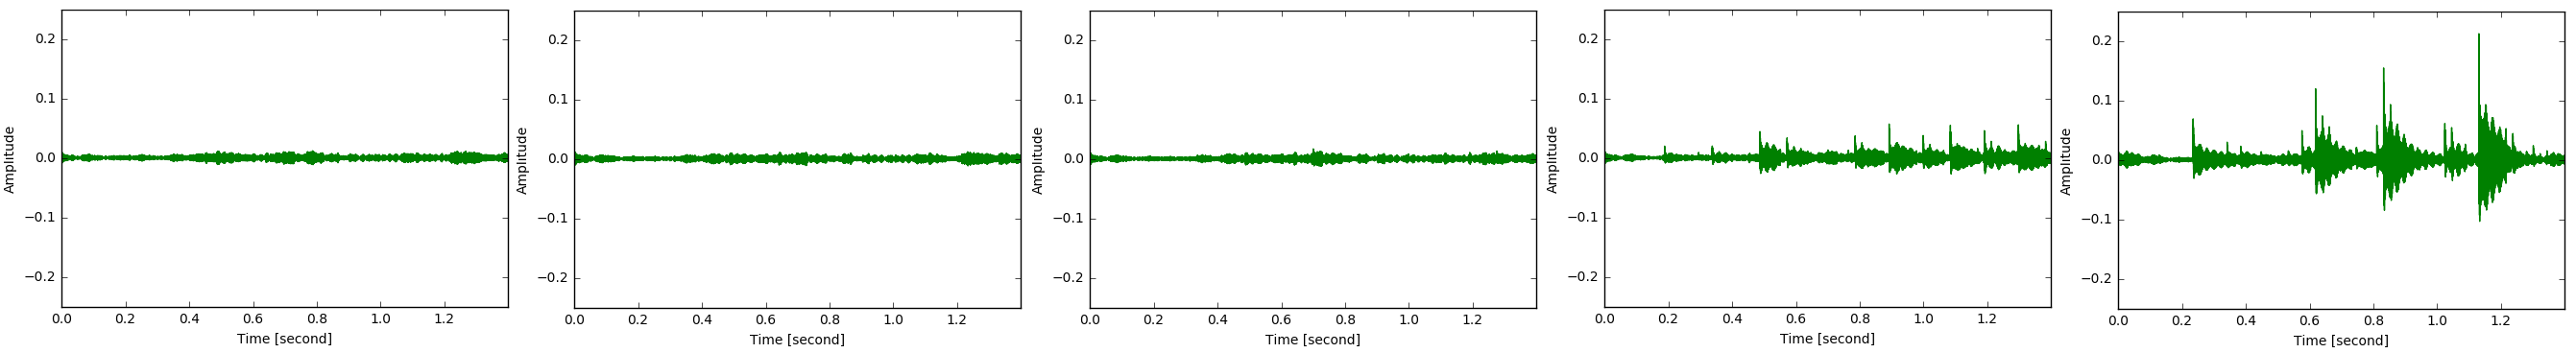
\includegraphics[width=\textwidth]{specs/sph_roughness.png}
      \caption{Waveforms of a bottle object with surface roughness variation (from very smooth to very rough), rolling on a platform.}
      \label{fig:bottle_rough}
\end{figure}

\begin{figure}[H]
  \centering
    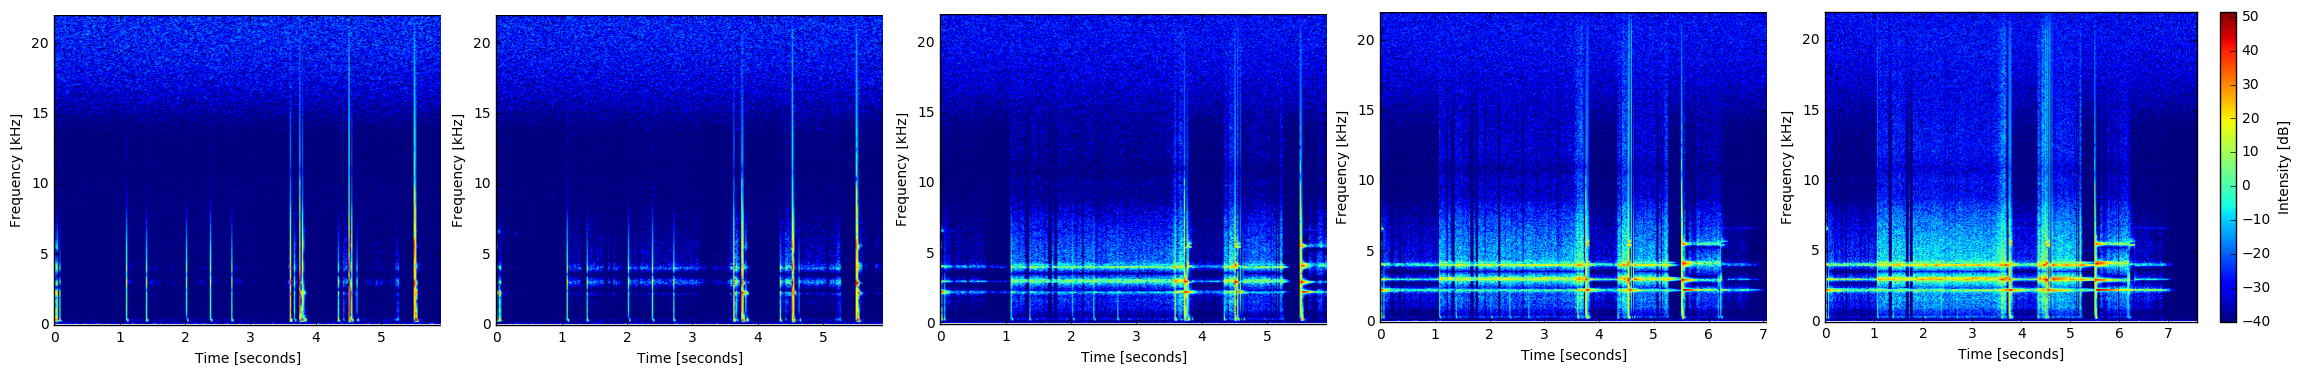
\includegraphics[width=\textwidth]{specs/bottle_materials.png}
      \caption{Spectrograms of a bottle object with material variation (plastic, wooden, ceramic, glass and metallic respectively).}
      \label{fig:bottle_materials}
\end{figure}

\paragraph{Integration of the tool\\}

The tool's \gls{UI} has been implemented similar to Unity\textsuperscript{\textregistered}'s \gls{UI} so that game developers feel familiar with the controls and can use it without having to learn how to use a third party audio solution. The goal is to assign a procedurally generated sound to an object in the game scene as easily  as one can apply a material texture. Therefore, not only sound designers who desire more realistic sound effects are targeted, but also game developers who are used to the Unity\textsuperscript{\textregistered} Editor and have no further sound design knowledge. Some game developers were consulted regarding the integration of the tool within the game engine and endorsed this approach.

As a side note, it is important for the designer to remember to press the \textit{``Apply''} button, on the prefab, every time a change is made, otherwise it will be undone. 



\subsection{CPU demands}\label{subsec: cpu}
Synthesizing sounds for applications in real-time instead of using a large bank of prerecorded clips is a good solution for the data storage problem. This is particularly a critical issue for standalone devices such as the HoloLens headset which presents storage and memory restrictions. Audio systems require sufficient CPU to operate when usually they have to compete with other systems such as graphics, physics and artificial intelligence (AI) \cite{lloyd2011sound}. 

In the tool presented in this paper however, when profiling a demonstration of a wine bottle rolling down a number of oblique platforms (seen in figure \ref{fig:test_sc2}) using the \textit{Profiler Window} of Unity\textsuperscript{\textregistered} Editor, it can be seen that except for the initialization stage where scripts consume CPU power, the rest of the demonstration remains stable in performance and at around $100 fps$ (figure \ref{fig:profile}). This performance test was held on a laptop with 4 Intel\textregistered\ Core\texttrademark\ i7-6700HQ CPUs running at 2.60GHz, each with 2 hardware threads.

\begin{figure}[H]
  \centering
    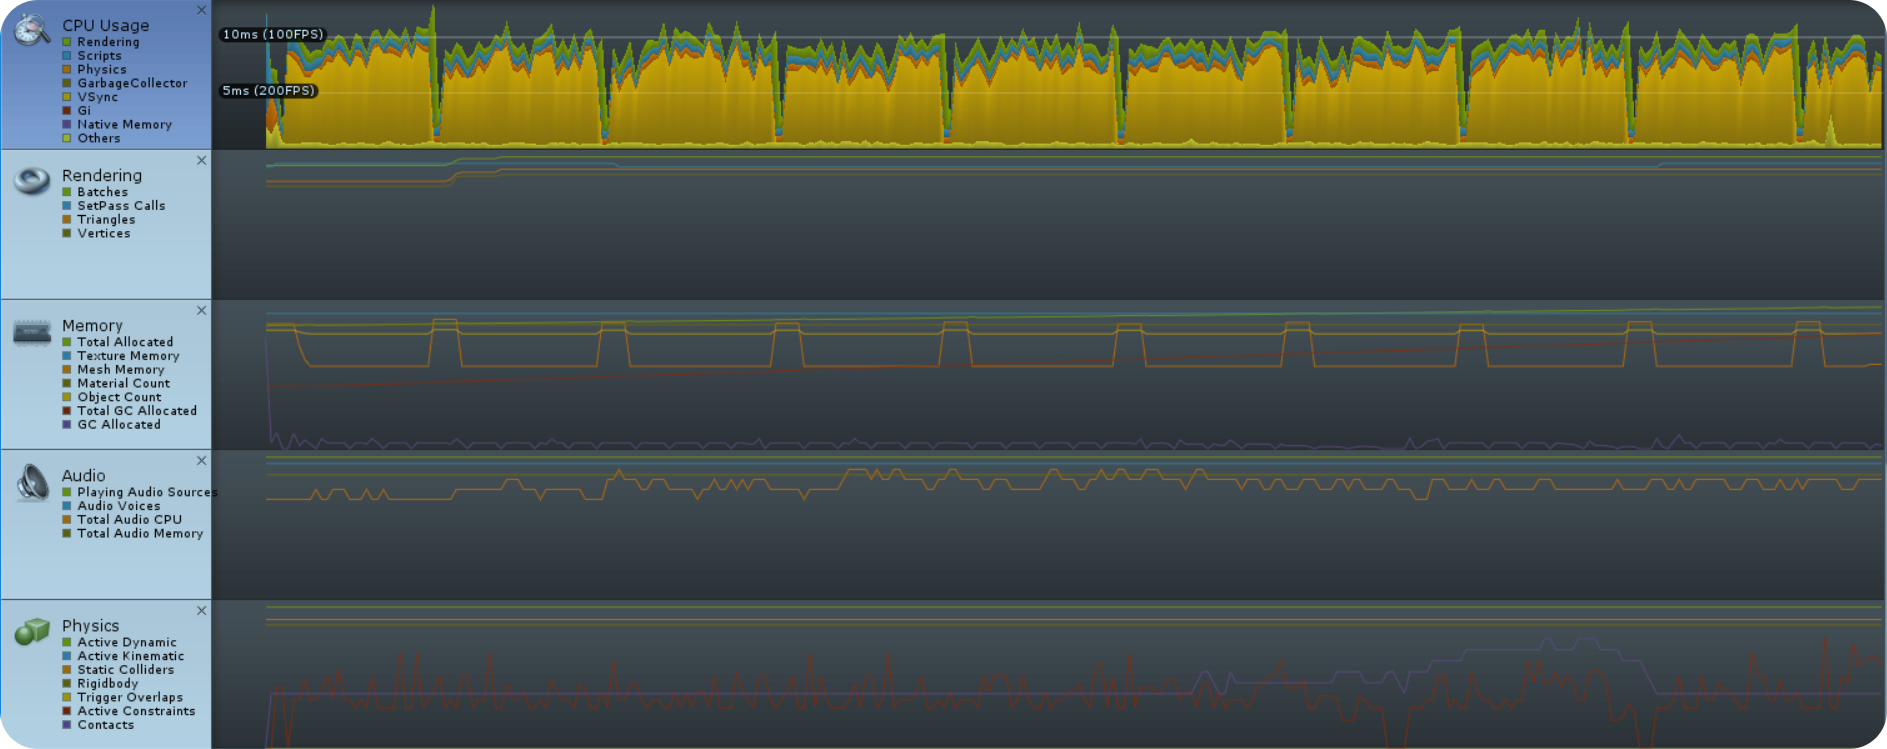
\includegraphics[width=\textwidth]{profiling1_r.PNG}
      \caption{The profiler view of Unity\textsuperscript{\textregistered} Editor when a wine bottle rolls down a number of platforms.}
      \label{fig:profile}
\end{figure} 

When testing the limits of the tool, it was found that for the filter-based method a total of 16 objects can be active at the same time before the audio gets distorted. The corresponding number for the sinusoidal method is 12 objects. This could be due to the fact that the latter method completes more calculations when computing the amplitude envelopes of each impact sound. Those numbers were obtained on the laptop mentioned above, using the \textit{Unity\textsuperscript{\textregistered} Audio Profiler window} and represent the amount of ``Playing Audio Sources'' without the ``Total Audio CPU'' exceeding $100\%$ (see figure \ref{fig:audio_profile}).

Overall, most of the calculations happen at the start of the application, leaving only the identification of the object and its corresponding data to be sent to the audio chain in real-time.  Therefore, it can be said that procedural audio does not consume more calculation power than is provided for audio in game and application productions.   

\begin{figure}[H]
  \centering
    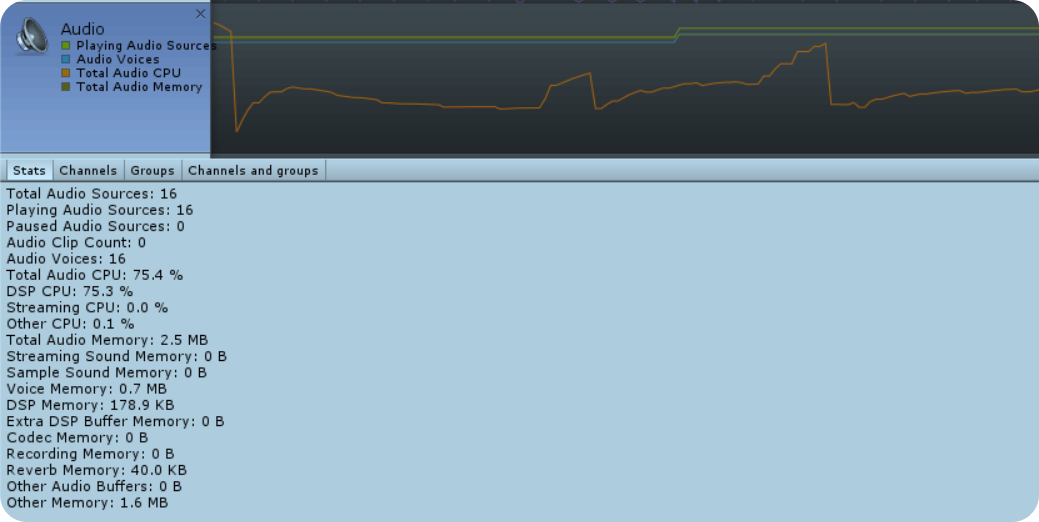
\includegraphics[width=\textwidth]{audio_profile_r.PNG}
      \caption{The audio profiler view of Unity\textsuperscript{\textregistered} Editor when a total of 16 objects are enabled in the scene using the filter-based method for audio synthesis.}
      \label{fig:audio_profile}
\end{figure}

\subsection{Which Synthesis Method Is Better?}
After analyzing the results of the listening experiments from section \ref{sec:testresults}, it can be stated that there is not much difference between the two methods used to synthesize modal sounds. Each object, with its characteristic physical attributes, gives slightly different results. However, a division per material is possible to arise as seen in table \ref{tab:method_mat} although it no clear conclusions can be extracted from it. A synthesis method does not seem to give better results over another one depending on the damping of the material.

In appendix \ref{ap:spectrograms}, the spectrograms for one object of each material examined in this work are shown. Although there are differences, both synthesis methods follow similar behavior in the frequency and time domain to the recordings.

From a more practical point of view, the sinusoidal synthesis method integrates less well in an environment in which multiple sounds can be triggered in a short lapse of time. This method uses an amplitude envelope that changes over time to simulate the sound decay. The problem arises when a second sound is triggered while the previous one's ``tail'' has not yet finished ``ringing''. This leads to the abrupt stop of the first sound in detriment of the second. To correct this three envelopes have been implemented so that up to three sounds coming from the same object can be played at the same time. On the other hand this issue does not occur with the filter-based method which is able to handle several impulses at a time. For this same reason this method is chosen for rolling and scratching sounds as these imply numerous micro-impacts in a short time lapse. Therefore, this method integrates better in interactive applications which demand a high degree of versatility as far as contact sounds are concerned. Moreover,  the filter-based synthesis allows more spatialized audio sources to be active before being distorted than the sinusoidal method. It can be therefore said that the filter-based method is overall more suitable for interactive applications due to its flexibility and integration.


\section{Discussion}
In this section, an overall discussion about the tool's usability is made and future work directions are considered.

\subsection{What is new?}
The main novelty of the tool presented is that it enables the generation and intuitive manipulation of physics-based procedural sounds within a game engine. This is based on the goal to bridge university research with industry by which often do not progress hand in hand.
Additionally, a study between two different sound synthesis methods, namely \textit{Sinusoidal Additive Synthesis} and \textit{Filter-based Modal Synthesis} is carried out. The sounds produced by these methods were tested by performing audio perception experiments on a group of participants to find out whether one of them offers better results than the other.
The tool offers the possibility to synthesize three kind of contact sounds (impact, rolling and scratching) that can be controlled through high level parameters. All of this being available in a package that is easily integrated in Unity\textsuperscript{\textregistered} and ready-to-use for game developers. 

\subsection{Tool applications}
This tool can be used for the development of all sorts of games that include collisions and interaction with physical objects. They can vary from indoor \gls{AR} applications, \gls{VR} games or simulations, to open world environment games running on consoles. However, in its current form it is recommended to be used for indoor games, since all prefabs available are every day object found in a kitchen. Designers are highly advised to use it for \gls{AR} applications, in which the synthesized sounds' realism is compared to the sounds of the real world.

\subsection{Why can it be used in AR/VR?}
Virtual and augmented reality are becoming more and more widespread technologies. There are multiple applications where they can prove to be useful both in everyday life and entertainment. Focusing on \gls{AR}, this thesis' goal is to develop a framework for sounds produced by the interaction of objects. The sounds are designed to be realistic and physics-based so they can adapt into an \gls{AR} environment where real sounds and virtual ones coexist. Furthermore, thanks to the memory storage solution that procedural audio entails, it is possible to use our tool on portable devices with small storage space.

\gls{VR} devices, although they do not have storage problems since they are connected to PCs to work, they, as well as \gls{AR}, require flexible sounds that can adapt to any virtual scenario. In addition the tool allows sound spatialization which suits both technologies that simulate three dimensional worlds.

\subsection{Future work}


The implemented tool is able to transfer an object's physical attributes from recordings to synthesized sounds. However, certain changes could be made to improve the accuracy of the synthesis and its cost from a computational point of view.

To improve the realism of the sound produced by a vibrating object in a virtual scene sound radiation should be taken into account. As described in \cite{corbett2007timbrefields}, not only the location of the excitation point controls the timbre of the sound, but also the location of the listener. The radiation, namely the energy transferred to the listener's ear, depends on his location and it is calculated through the \textit{acoustic transfer function}. Adding this component would enhance significantly the feeling of immersion in the virtual environment.

Another improvement that could be done is the early spatialization of the sound in the synthesis process. More specifically, instead of dividing the process into two steps, namely the synthesis of the monophonic sound and then the spatialization, another option would be to do it at the same time as seen in \cite{verron2010synthese}, using the location of the object and listener. This approach would save calculation power for sounds that are very far away from the listener. The concept of dynamic level of audio is interesting for the creation of sounds taht woulde present a variable cost as stated by Farnell \cite{farnell2010designing}. Similarly to the compression of audio like with the MP3 format, less resources would be used as the sounding object moves further from the listener. This can be accomplished by cascading the band-pass filters of the filter-based method with spatial filters.    

Furthermore, some future work regarding sound propagation in rooms and occlusion produced by the environment could be done. Some papers have studied the sounds produced by objects that break into smaller pieces which could be another direction to go \cite{zheng2010rigid}.


